\documentclass[aspectratio=169,xcolor=dvipsnames,t]{beamer}
\usepackage[utf8]{inputenc}

\usepackage{amssymb}
\usepackage{amsmath}
\usepackage{rotating}
\usepackage{graphicx}
\usepackage[mathscr]{euscript}
\usepackage[dvipsnames,svgnames,table]{xcolor}
\usepackage{multicol}
\usepackage{multirow}
\usepackage{physics}
\usepackage[version=4]{mhchem}
\usepackage[spanish,es-nodecimaldot,es-tabla]{babel}
\usepackage{parskip}
\usepackage{hyperref}
\usepackage{csquotes}
\usepackage{wrapfig}
\usepackage{ragged2e}
\justifying

\usepackage{etoolbox}
\usepackage{textcase}
\makeatletter
\patchcmd{\beamer@Section}{\Section}{\Section{\MakeTextUppercase}{}{}}{}{}
\patchcmd{\beamer@Subsection}{\Subsection}{\Subsection{\MakeTextUppercase}{}{}}{}{}
\makeatother

\usepackage[backend=biber,citestyle=numeric-comp,bibstyle=apa,sorting=none]{biblatex}
\bibliography{ref}
\makeatletter
\RequireBibliographyStyle{numeric}
\makeatother

\newcommand{\be}{\begin{equation*}}
\newcommand{\ee}{\end{equation*}}
\newcommand{\ble}[1]{\begin{equation} \label{#1}}
\newcommand{\bae}{\begin{eqnarray}}
\newcommand{\eae}{\end{eqnarray}}
\newcommand{\pl}{\left(}
\newcommand{\pr}{\right)}
\newcommand{\kl}{\left[}
\newcommand{\kr}{\right]}

\setbeamertemplate{footline}[frame number]

\usetheme{Arguelles}

%%%%%%%%%%%%%%%%%%%% Opciones título %%%%%%%%%%%%%%%

\title{Algoritmos de planificación del tratamiento: cálculos de dosis de fotones}
\subtitle{Khan's Treatment Planning in Radiation Oncology \tiny{\cite{Khans}}}

\date{\today}
\author{Christopher López Ruiz}
\institute{Instituto Nacional de Cancerología}

%%%%%%%%%%%%%%%%%%%%%%%%%%%%%%%%%%%%%%%%%%%%%%%%%%%%%%%%%%%%%%%%%%%

\begin{document}

\frame[plain,bg=fondo.jpg]{\titlepage}

\Section{Introduccion}

\begin{frame}[standout]
      \centering\LARGE
      \textbf{\itshape\scshape Introducción}
\end{frame}

\begin{frame}

    \vspace{0.45cm}

    \begin{wrapfigure}{r}{0.3\textwidth}
        \centering
        \includegraphics[width=0.45\textwidth,angle=90]{tarjeta.jpg}
    \end{wrapfigure}

    \textbf{Historia}
    
    \begin{itemize}
        \item Los sistemas computarizados de planificación del tratamiento se han utilizado en la \textbf{planificación de la radioterapia desde la década de 1950}.
        \item El primer algoritmo informático utilizado se atribuyó a Tsien, quien \textbf{utilizó tarjetas perforadas para almacenar distribuciones de isodosis y permitir la adición de múltiples haces}.
        \item Los avances en la \textbf{velocidad de las computadoras y el desarrollo de algoritmos han mejorado} enormemente nuestra \textbf{capacidad para predecir las distribuciones de dosis de fotones en los pacientes}.
    \end{itemize}

\end{frame}

\begin{frame}
      
    En 1987 el \textbf{informe 42 de la ICRU} hace el primer intento de \textbf{clasificar los algoritmos de planificación informática}.

    \begin{figure}[h]
        \centering
        \includegraphics[width=0.6\textwidth]{tiposa.pdf}
    \end{figure}

    \textit{Empíricos}
    
    \begin{itemize}
        \item \textbf{Primeros algoritmos} se desarrollaron utilizando como \textbf{entrada datos de haces clínicos medidos en un phantom de agua plana.} Luego se hicieron \textbf{correcciones} para incorporar varios efectos.
        \item Con el tiempo, se incorporaron \textbf{factores de corrección de la heterogeneidad del paciente}, pero se aplicaron después, es decir, \textbf{después de realizar cálculos basados en agua asumiendo una geometría homogénea del paciente}.
    \end{itemize}

\end{frame}

\begin{frame}
    
    \begin{itemize}
        \item La mayor parte de este desarrollo se produjo \textbf{antes de la llegada de la CT}.
        \item Con el tiempo, la \textbf{utilización comercial de algoritmos empíricos se desvaneció.}
    \end{itemize}

    \begin{wrapfigure}{l}{0.4\textwidth}
        \centering
        \includegraphics[width=0.4\textwidth]{ct.jpeg}
    \end{wrapfigure}

    \textit{Basados en modelos}

    \begin{itemize}
        \item En \textbf{1990}, la \textbf{radioterapia conformada tridimensional (3D CRT) comenzó a utilizar datos de imágenes de CT} específicos del paciente en el proceso de planificación.
        \item Al principio \textbf{se limitaba a una simulación virtual}. Ya que \textbf{aún no estaban disponibles algoritmos informáticos} que pudieran incorporar la \textbf{información de densidad volumétrica} y calcular \textbf{distribuciones de dosis} tridimensionales en un período de tiempo razonable.
    \end{itemize}
\end{frame}

\begin{frame}

    \vspace{0.6cm}

    \begin{itemize}
        \item Para utilizar plenamente esta nueva información, fue necesario \textbf{desarrollar nuevos algoritmos que pudieran incorporar con mayor precisión variaciones en la anatomía de cada paciente}.
        \item Como resultado, los \textbf{sistemas comerciales de planificación de tratamientos han pasado a métodos de cálculo de fotones basados en modelos.}
    \end{itemize}

    \vspace{5pt}

    En este capítulo, se describen \textbf{tres modelos de cálculo de fotones que se utilizan actualmente en clínicas de radioterapia}. 
    
    Los modelos de cálculo de fotones son \textbf{un área de desarrollo continuo y es probable que la implementación de uno o más de estos modelos por parte de cada proveedor comercial difiera en muchos aspectos}. Sin embargo, la intención es \textbf{proporcionar una comprensión básica de los principios detrás de estos algoritmos}.

\end{frame}

\Section{La representacion del paciente}

\begin{frame}[standout]
      \centering\LARGE
      \textbf{\itshape\scshape La representación del paciente para la planificación de la dosis}
\end{frame}

\begin{frame}

    \textbf{Inicialmente}, los pacientes eran considerados como un \textbf{phantom de agua plana} con un \textbf{SSD} y una \textbf{profundidad específicos} para su uso en \textbf{cálculos de dosis simples o de unidades de monitorización}.

    El desarrollo de \textbf{herramientas de contorno externo} ayudó al planificador del tratamiento a determinar \textbf{distribuciones de dosis específicas para el paciente}. Dichos procedimientos dieron como resultado que el \textbf{paciente fuera representado como una composición homogénea} (es decir, agua), pero \textbf{permitieron la aplicación de correcciones superficiales al cálculo}.

    \begin{figure}[h]
        \centering
        \includegraphics[width=0.55\textwidth]{p1.pdf}
    \end{figure}

\end{frame}

\begin{frame}

    Las \textbf{heterogeneidades} de los pacientes \textbf{podrían representarse} de formas sencillas, como \textbf{utilizando contornos internos con densidades asignadas}.

    La densidad electrónica a asignar a la región podría \textbf{inferirse de los atlas de CT} o, si están disponibles, del \textbf{número medio de CT específico del paciente dentro de la estructura contorneada}.

    El \textbf{problema} con este enfoque fue que \textbf{tejidos} como el pulmón y el hueso \textbf{no son homogéneos en sí mismos y sus variaciones de densidad no se tendrían en cuenta al utilizar este enfoque}.

\end{frame}

\begin{frame}

      \frametitle{Método Monte Carlo \tiny{\cite{IBM}}}

      \vspace{0.5cm}

      \begin{wrapfigure}{r}{0.5\textwidth}
            \centering
            \includegraphics[width=0.5\textwidth]{ruleta.jpg}
      \end{wrapfigure}

      Es una \textbf{técnica matemática} que se utiliza para estimar los \textbf{posibles resultados} de un evento incierto.
      
      Inventado por \textbf{John von Neumann} y \textbf{Stanislaw Ulam} para mejorar la toma de decisiones en condiciones inciertas.
      
      Lleva el nombre de una conocida \textbf{ciudad de casinos}.

      Desde su introducción han evaluado el \textbf{impacto del riesgo} en muchos escenarios de la \textbf{vida real}.
\end{frame}


\begin{frame}
      \textbf{II. La cavidad es grande comparada con el alcance de los electrones involucrados}

      \begin{itemize}
            \item Definido con el cociente del coeficiente de absorción de energía
            \item Asumir que la cavidad no perturba la fluencia fotones, i.e. $(\Phi_k)_{med} = (\Phi_k)_{det}$
      \end{itemize}

      \be
      f_{med,det}(Q) = \frac{\int_{0}^{k_{max}} [\Phi_k]_{med} [\mu_{en}(k)/\rho]_{med} \, dk}{\int_{0}^{k_{max}} [\Phi_k]_{med} [\mu_{en}(k)/\rho]_{det} \, dk} = [\mu_{en}/\rho]_{med,det}
      \ee
\end{frame}

\Section{Calculo Monte Carlo de cantidades dosimetricas}

\begin{frame}[standout]
      \centering\LARGE
      \textbf{\itshape\scshape Cálculo Monte Carlo de cantidades dosimétricas}
\end{frame}

\begin{frame}
      \frametitle{Cocientes de poder de frenado para dosimetría de referencia}

      El problema básicamente se restringe al \textbf{cálculo de la fluencia de partícula cargadas relevantes o de fotones, diferencial en energía}, puntuando \textit{espectros de longitud de pista}.

      Muchos de los avances de MC en este campo han estado relacionados con desarrollos en \textbf{algoritmos de transporte de electrones}, especialmente en presencia de límites de interfaz, donde los segmentos de longitud de pista pueden volverse tan cortos que las \textbf{múltiples teorías de dispersión ya no son válidas bajo la llamada técnica de historia condensada}.

      Muchos de los sistemas MC actuales incluyen dicha técnica, en lugar del tipo de simulación de \textbf{interacción por interacción (dispersión única)} que suele utilizarse para la simulación del transporte de baja energía.
\end{frame}

\Section{Conclusiones}

\begin{frame}[standout]
      \centering\LARGE
      \textbf{\itshape\scshape Conclusiones}
\end{frame}


\End
\begin{frame}[standout,bg=white.png]
      \centering
      \printbibliography
\end{frame}

\end{document}